%%
%% Automatically generated file from DocOnce source
%% (https://github.com/doconce/doconce/)
%% doconce format latex Catania.do.txt --latex_title_layout=beamer --latex_table_format=footnotesize --no_mako
%%
% #ifdef PTEX2TEX_EXPLANATION
%%
%% The file follows the ptex2tex extended LaTeX format, see
%% ptex2tex: https://code.google.com/p/ptex2tex/
%%
%% Run
%%      ptex2tex myfile
%% or
%%      doconce ptex2tex myfile
%%
%% to turn myfile.p.tex into an ordinary LaTeX file myfile.tex.
%% (The ptex2tex program: https://code.google.com/p/ptex2tex)
%% Many preprocess options can be added to ptex2tex or doconce ptex2tex
%%
%%      ptex2tex -DMINTED myfile
%%      doconce ptex2tex myfile envir=minted
%%
%% ptex2tex will typeset code environments according to a global or local
%% .ptex2tex.cfg configure file. doconce ptex2tex will typeset code
%% according to options on the command line (just type doconce ptex2tex to
%% see examples). If doconce ptex2tex has envir=minted, it enables the
%% minted style without needing -DMINTED.
% #endif

% #define PREAMBLE

% #ifdef PREAMBLE
%-------------------- begin preamble ----------------------

\documentclass[%
oneside,                 % oneside: electronic viewing, twoside: printing
final,                   % draft: marks overfull hboxes, figures with paths
10pt]{article}

\listfiles               %  print all files needed to compile this document

\usepackage{relsize,makeidx,color,setspace,amsmath,amsfonts,amssymb}
\usepackage[table]{xcolor}
\usepackage{bm,ltablex,microtype}

\usepackage[pdftex]{graphicx}

\usepackage[T1]{fontenc}
%\usepackage[latin1]{inputenc}
\usepackage{ucs}
\usepackage[utf8x]{inputenc}

\usepackage{lmodern}         % Latin Modern fonts derived from Computer Modern

% Hyperlinks in PDF:
\definecolor{linkcolor}{rgb}{0,0,0.4}
\usepackage{hyperref}
\hypersetup{
    breaklinks=true,
    colorlinks=true,
    linkcolor=linkcolor,
    urlcolor=linkcolor,
    citecolor=black,
    filecolor=black,
    %filecolor=blue,
    pdfmenubar=true,
    pdftoolbar=true,
    bookmarksdepth=3   % Uncomment (and tweak) for PDF bookmarks with more levels than the TOC
    }
%\hyperbaseurl{}   % hyperlinks are relative to this root

\setcounter{tocdepth}{2}  % levels in table of contents

% Tricks for having figures close to where they are defined:
% 1. define less restrictive rules for where to put figures
\setcounter{topnumber}{2}
\setcounter{bottomnumber}{2}
\setcounter{totalnumber}{4}
\renewcommand{\topfraction}{0.95}
\renewcommand{\bottomfraction}{0.95}
\renewcommand{\textfraction}{0}
\renewcommand{\floatpagefraction}{0.75}
% floatpagefraction must always be less than topfraction!
% 2. ensure all figures are flushed before next section
\usepackage[section]{placeins}
% 3. enable begin{figure}[H] (often leads to ugly pagebreaks)
%\usepackage{float}\restylefloat{figure}

\usepackage[framemethod=TikZ]{mdframed}

% --- begin definitions of admonition environments ---

% Admonition style "mdfbox" is an oval colored box based on mdframed
% "notice" admon
\colorlet{mdfbox_notice_background}{gray!5}
\newmdenv[
  skipabove=15pt,
  skipbelow=15pt,
  outerlinewidth=0,
  backgroundcolor=mdfbox_notice_background,
  linecolor=black,
  linewidth=2pt,       % frame thickness
  frametitlebackgroundcolor=mdfbox_notice_background,
  frametitlerule=true,
  frametitlefont=\normalfont\bfseries,
  shadow=false,        % frame shadow?
  shadowsize=11pt,
  leftmargin=0,
  rightmargin=0,
  roundcorner=5,
  needspace=0pt,
]{notice_mdfboxmdframed}

\newenvironment{notice_mdfboxadmon}[1][]{
\begin{notice_mdfboxmdframed}[frametitle=#1]
}
{
\end{notice_mdfboxmdframed}
}

% Admonition style "mdfbox" is an oval colored box based on mdframed
% "summary" admon
\colorlet{mdfbox_summary_background}{gray!5}
\newmdenv[
  skipabove=15pt,
  skipbelow=15pt,
  outerlinewidth=0,
  backgroundcolor=mdfbox_summary_background,
  linecolor=black,
  linewidth=2pt,       % frame thickness
  frametitlebackgroundcolor=mdfbox_summary_background,
  frametitlerule=true,
  frametitlefont=\normalfont\bfseries,
  shadow=false,        % frame shadow?
  shadowsize=11pt,
  leftmargin=0,
  rightmargin=0,
  roundcorner=5,
  needspace=0pt,
]{summary_mdfboxmdframed}

\newenvironment{summary_mdfboxadmon}[1][]{
\begin{summary_mdfboxmdframed}[frametitle=#1]
}
{
\end{summary_mdfboxmdframed}
}

% Admonition style "mdfbox" is an oval colored box based on mdframed
% "warning" admon
\colorlet{mdfbox_warning_background}{gray!5}
\newmdenv[
  skipabove=15pt,
  skipbelow=15pt,
  outerlinewidth=0,
  backgroundcolor=mdfbox_warning_background,
  linecolor=black,
  linewidth=2pt,       % frame thickness
  frametitlebackgroundcolor=mdfbox_warning_background,
  frametitlerule=true,
  frametitlefont=\normalfont\bfseries,
  shadow=false,        % frame shadow?
  shadowsize=11pt,
  leftmargin=0,
  rightmargin=0,
  roundcorner=5,
  needspace=0pt,
]{warning_mdfboxmdframed}

\newenvironment{warning_mdfboxadmon}[1][]{
\begin{warning_mdfboxmdframed}[frametitle=#1]
}
{
\end{warning_mdfboxmdframed}
}

% Admonition style "mdfbox" is an oval colored box based on mdframed
% "question" admon
\colorlet{mdfbox_question_background}{gray!5}
\newmdenv[
  skipabove=15pt,
  skipbelow=15pt,
  outerlinewidth=0,
  backgroundcolor=mdfbox_question_background,
  linecolor=black,
  linewidth=2pt,       % frame thickness
  frametitlebackgroundcolor=mdfbox_question_background,
  frametitlerule=true,
  frametitlefont=\normalfont\bfseries,
  shadow=false,        % frame shadow?
  shadowsize=11pt,
  leftmargin=0,
  rightmargin=0,
  roundcorner=5,
  needspace=0pt,
]{question_mdfboxmdframed}

\newenvironment{question_mdfboxadmon}[1][]{
\begin{question_mdfboxmdframed}[frametitle=#1]
}
{
\end{question_mdfboxmdframed}
}

% Admonition style "mdfbox" is an oval colored box based on mdframed
% "block" admon
\colorlet{mdfbox_block_background}{gray!5}
\newmdenv[
  skipabove=15pt,
  skipbelow=15pt,
  outerlinewidth=0,
  backgroundcolor=mdfbox_block_background,
  linecolor=black,
  linewidth=2pt,       % frame thickness
  frametitlebackgroundcolor=mdfbox_block_background,
  frametitlerule=true,
  frametitlefont=\normalfont\bfseries,
  shadow=false,        % frame shadow?
  shadowsize=11pt,
  leftmargin=0,
  rightmargin=0,
  roundcorner=5,
  needspace=0pt,
]{block_mdfboxmdframed}

\newenvironment{block_mdfboxadmon}[1][]{
\begin{block_mdfboxmdframed}[frametitle=#1]
}
{
\end{block_mdfboxmdframed}
}

% --- end of definitions of admonition environments ---

% prevent orhpans and widows
\clubpenalty = 10000
\widowpenalty = 10000

% --- end of standard preamble for documents ---


% insert custom LaTeX commands...

\raggedbottom
\makeindex

%-------------------- end preamble ----------------------

\begin{document}

% matching end for #ifdef PREAMBLE
% #endif

\newcommand{\exercisesection}[1]{\subsection*{#1}}


% ------------------- main content ----------------------



% ----------------- title -------------------------

\title{Artificial intelligence and machine learning in physics }

% ----------------- author(s) -------------------------

\author{Morten Hjorth-Jensen\inst{1}}
\institute{Department of Physics and Astronomy and FRIB, Michigan State University, USA, and Department of Physics and Center for Computing in Science Education, University of Oslo, Norway\inst{1}}
% ----------------- end author(s) -------------------------

\date{Department of Physics and Astronomy colloquium, University of Catania and celebrating MARCELLO BALDO'S 80th birthday
% <optional titlepage figure>
% <optional copyright>
}

% !split
\subsection{What is this talk about?}
\begin{block}{}
The main emphasis is to give you a short and pedestrian introduction to the whys and hows we can use (with several examples) machine learning methods
in physics. And why this could (or should) be of interest. 
\end{block}

\begin{block}{Additional info }
Parts of this talk are based on \href{{https://journals.aps.org/rmp/abstract/10.1103/RevModPhys.94.031003}}{Artificial Intelligence and Machine Learning in Nuclear Physics, Amber Boehnlein et al., Reviews Modern of Physics 94, 031003 (2022)} 
\end{block}

\begin{block}{}
These slides at \href{{https://mhjensenseminars.github.io/MachineLearningTalk/doc/web/overview.html}}{\nolinkurl{https://mhjensenseminars.github.io/MachineLearningTalk/doc/web/overview.html}}
\end{block}

% !split
\subsection{Thanks to many}

Jane Kim (MSU), Julie Butler (MSU), Patrick Cook (MSU), Danny Jammooa (MSU), Daniel Bazin (MSU), Dean Lee (MSU), Witek Nazarewicz (MSU), Michelle Kuchera (Davidson College), Even Nordhagen (UiO), Robert Solli (UiO, Expert Analytics), Bryce Fore (ANL), Alessandro Lovato (ANL), Stefano Gandolfi (LANL), Francesco Pederiva (UniTN), and Giuseppe Carleo (EPFL). 
Niyaz Beysengulov and Johannes Pollanen (experiment, MSU); Zachary Stewart, Jared Weidman, and Angela Wilson (quantum chemistry, MSU)
Jonas Flaten, Oskar, Leinonen, Øyvind Sigmundson Schøyen, Stian Dysthe Bilek, and Håkon Emil Kristiansen (UiO). Marianne Bathen and Lasse Vines (experiments (UiO). Excuses to those I have omitted.

% !split
\subsection{One of the first many-body workshops at the ECT$*$, Trento summer 1997}

\vspace{6mm}

% inline figure
\centerline{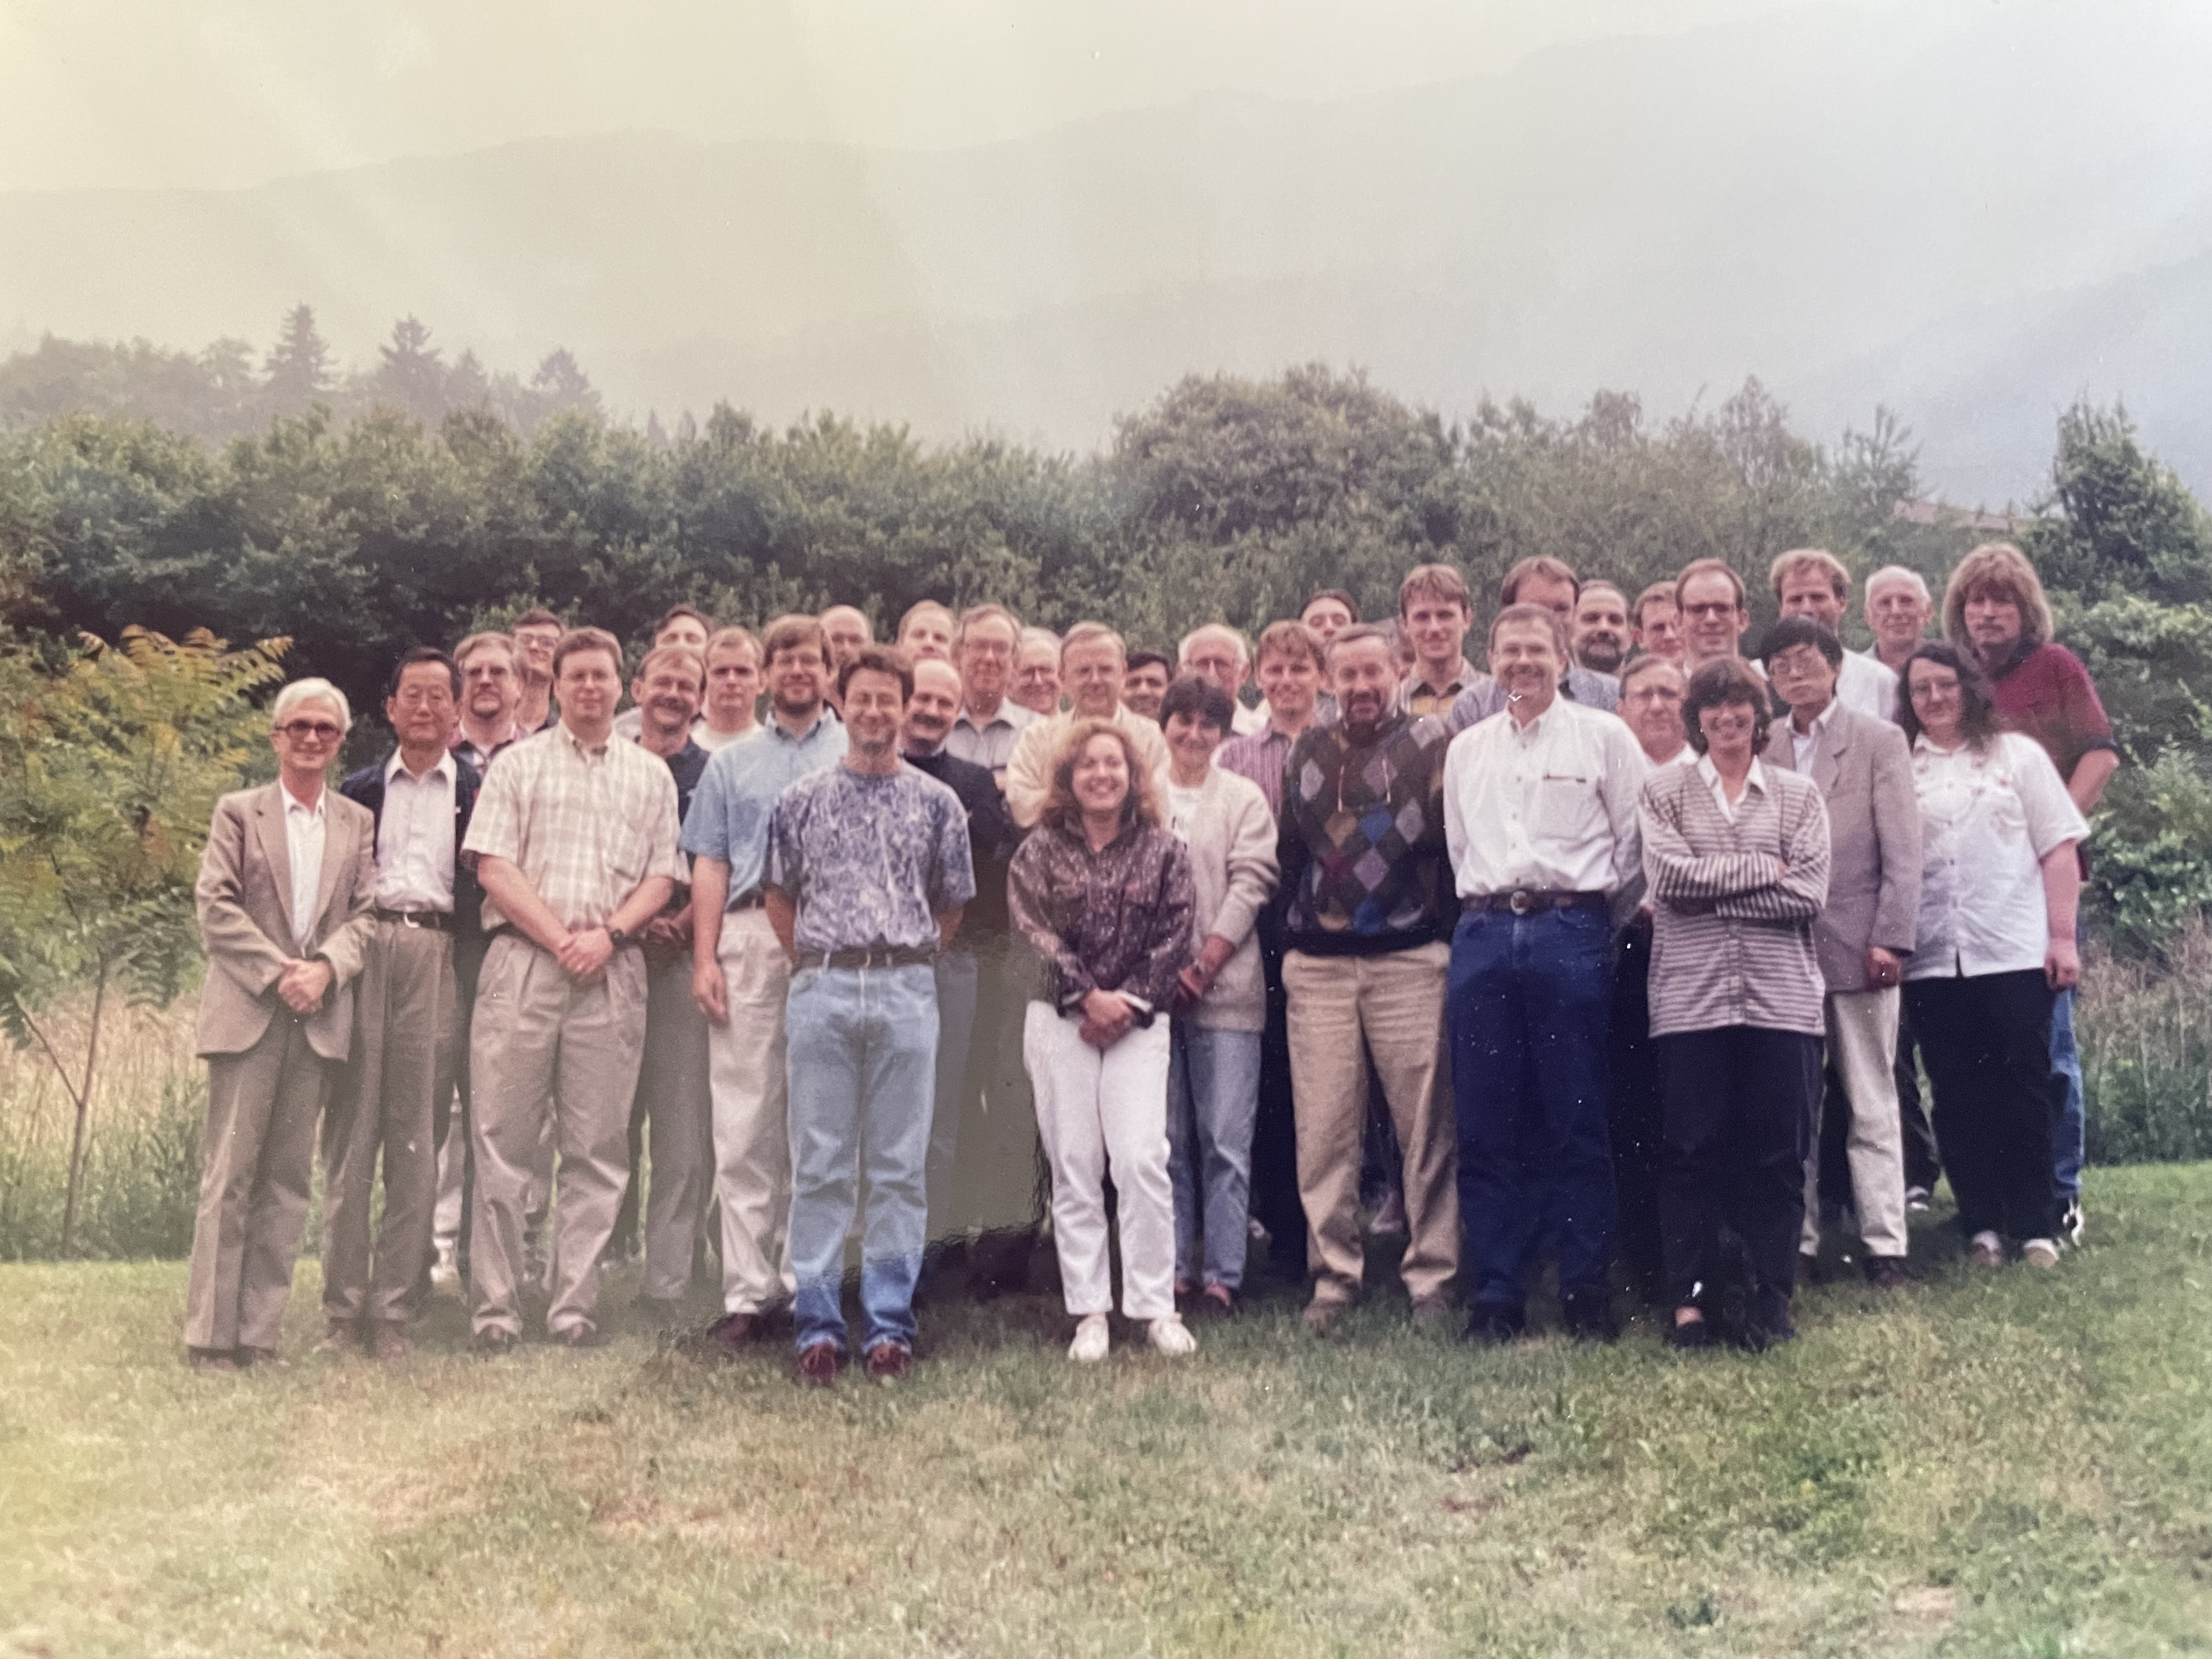
\includegraphics[width=1.0\linewidth]{Photos/manybody1997.jpeg}}

\vspace{6mm}

% !split
\subsection{Pairing in dense matter}

\vspace{6mm}

% inline figure
\centerline{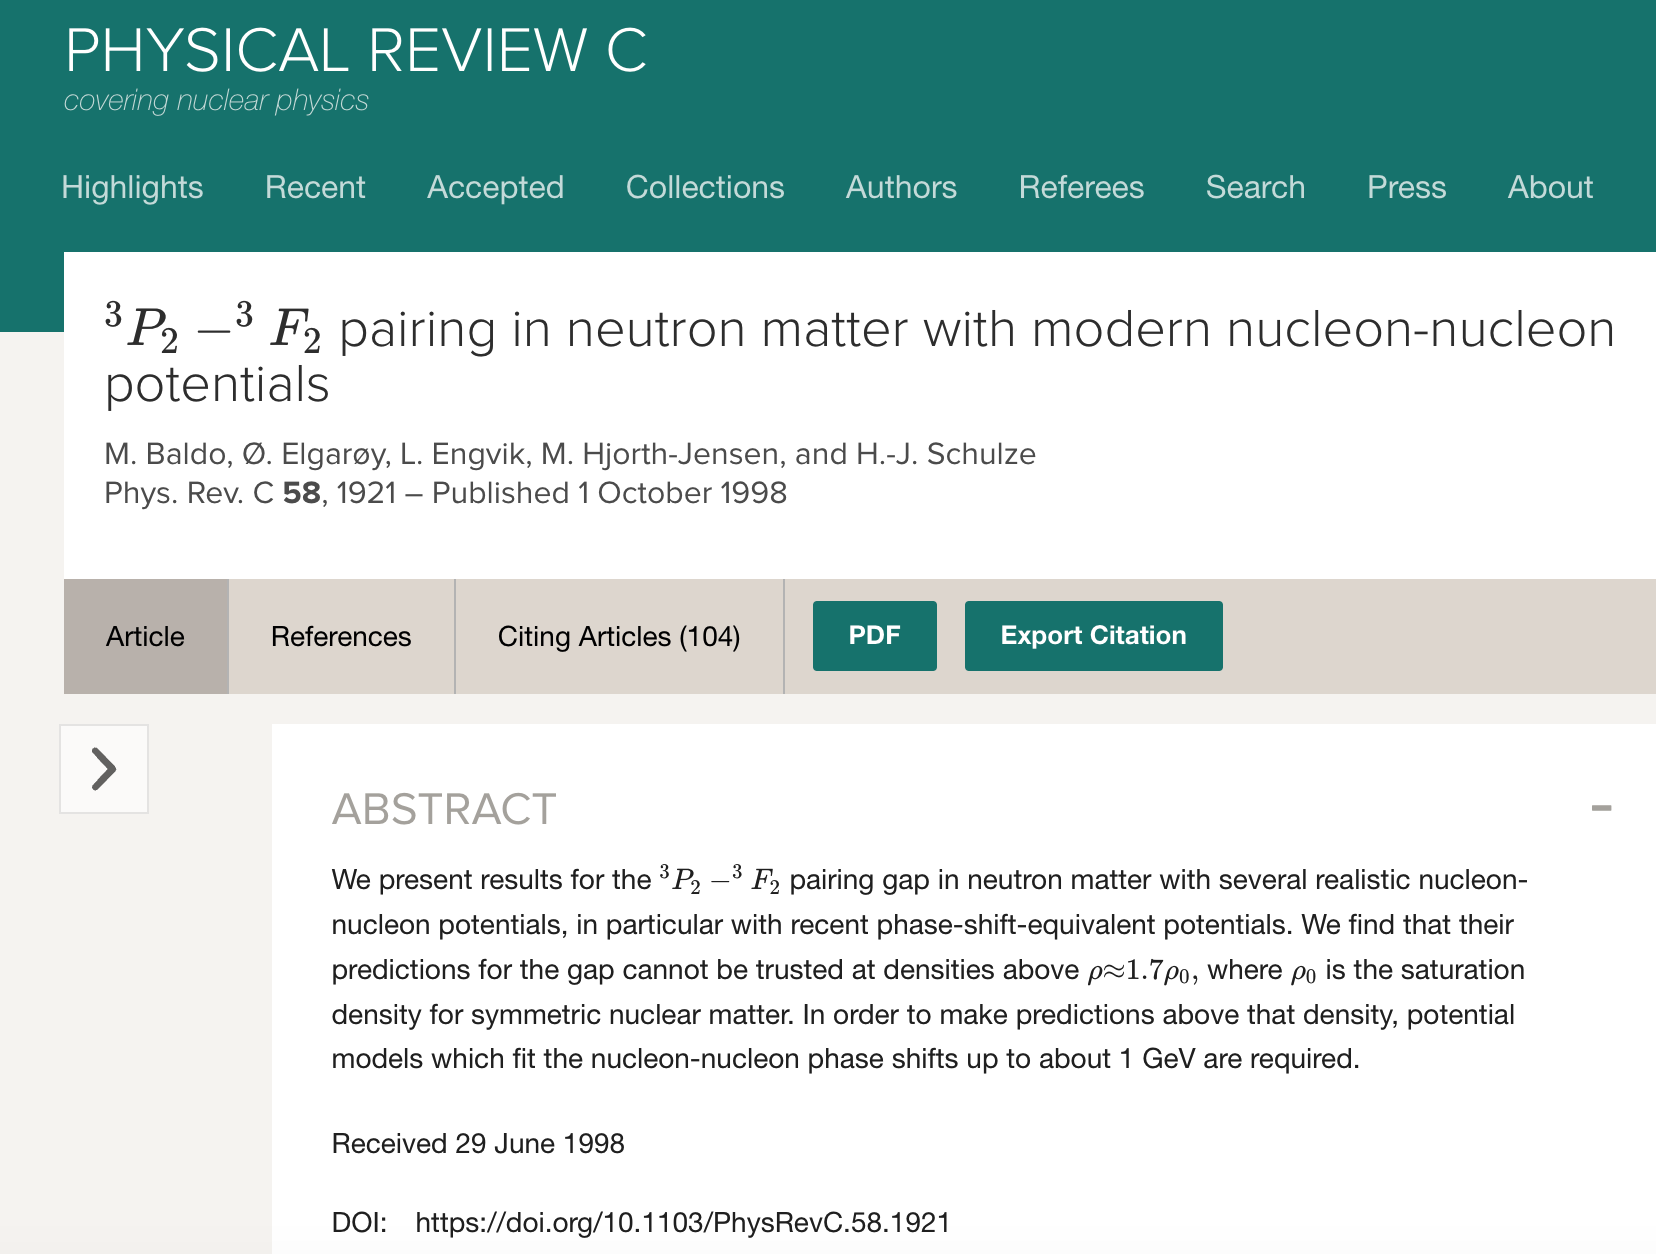
\includegraphics[width=1.0\linewidth]{figures/paperbaldo.png}}

\vspace{6mm}

% !split
\subsection{AI/ML and some statements you may have heard (and what do they mean?)}

\begin{enumerate}
\item Fei-Fei Li on ImageNet: \textbf{map out the entire world of objects} (\href{{https://cacm.acm.org/news/219702-the-data-that-transformed-ai-research-and-possibly-the-world/fulltext}}{The data that transformed AI research})

\item Russell and Norvig in their popular textbook: \textbf{relevant to any intellectual task; it is truly a universal field} (\href{{http://aima.cs.berkeley.edu/}}{Artificial Intelligence, A modern approach})

\item Woody Bledsoe puts it more bluntly: \textbf{in the long run, AI is the only science} (quoted in Pamilla McCorduck, \href{{https://www.pamelamccorduck.com/machines-who-think}}{Machines who think})
\end{enumerate}

\noindent
If you wish to have a critical read on AI/ML from a societal point of view, see \href{{https://www.katecrawford.net/}}{Kate Crawford's recent text Atlas of AI}. See also \href{{https://www.nationaldefensemagazine.org/articles/2023/3/24/ukraine-a-living-lab-for-ai-warfare}}{\nolinkurl{https://www.nationaldefensemagazine.org/articles/2023/3/24/ukraine-a-living-lab-for-ai-warfare}}

\textbf{Here: with AI/ML we intend a collection of machine learning methods with an emphasis on statistical learning and data analysis}

% !split
\subsection{Types of machine learning}

\begin{block}{}
The approaches to machine learning are many, but are often split into two main categories. 
In \emph{supervised learning} we know the answer to a problem,
and let the computer deduce the logic behind it. On the other hand, \emph{unsupervised learning}
is a method for finding patterns and relationship in data sets without any prior knowledge of the system.

An emerging  third category is  \emph{reinforcement learning}. This is a paradigm 
of learning inspired by behavioural psychology, where learning is achieved by trial-and-error, 
solely from rewards and punishment.
\end{block}

% !split
\subsection{Main categories}
\begin{block}{}
Another way to categorize machine learning tasks is to consider the desired output of a system.
Some of the most common tasks are:

\begin{itemize}
  \item Classification: Outputs are divided into two or more classes. The goal is to   produce a model that assigns inputs into one of these classes. An example is to identify  digits based on pictures of hand-written ones. Classification is typically supervised learning.

  \item Regression: Finding a functional relationship between an input data set and a reference data set.   The goal is to construct a function that maps input data to continuous output values.

  \item Clustering: Data are divided into groups with certain common traits, without knowing the different groups beforehand.  It is thus a form of unsupervised learning.
\end{itemize}

\noindent
\end{block}

% !split
\subsection{The plethora  of machine learning algorithms/methods}

\begin{enumerate}
\item Deep learning: Neural Networks (NN), Convolutional NN, Recurrent NN, Boltzmann machines, autoencoders and variational autoencoders  and generative adversarial networks, generative models 

\item Bayesian statistics and Bayesian Machine Learning, Bayesian experimental design, Bayesian Regression models, Bayesian neural networks, Gaussian processes and much more

\item Dimensionality reduction (Principal component analysis), Clustering Methods and more

\item Ensemble Methods, Random forests, bagging and voting methods, gradient boosting approaches 

\item Linear and logistic regression, Kernel methods, support vector machines and more

\item Reinforcement Learning; Transfer Learning and more 
\end{enumerate}

\noindent
% !split
\subsection{What are the basic ingredients?}
\begin{block}{}
Almost every problem in ML and data science starts with the same ingredients:
\begin{itemize}
\item The dataset $\mathbf{x}$ (could be some observable quantity of the system we are studying)

\item A model which is a function of a set of parameters $\mathbf{\alpha}$ that relates to the dataset, say a likelihood  function $p(\mathbf{x}\vert \mathbf{\alpha})$ or just a simple model $f(\mathbf{\alpha})$

\item A so-called \textbf{loss/cost/risk} function $\mathcal{C} (\mathbf{x}, f(\mathbf{\alpha}))$ which allows us to decide how well our model represents the dataset. 
\end{itemize}

\noindent
We seek to minimize the function $\mathcal{C} (\mathbf{x}, f(\mathbf{\alpha}))$ by finding the parameter values which minimize $\mathcal{C}$. This leads to  various minimization algorithms. It may surprise many, but at the heart of all machine learning algortihms there is an optimization problem. 
\end{block}

% !split
\subsection{Low-level machine lerning, the family of ordinary least squares methods}

Our data which we want to apply a machine learning method on, consist
of a set of inputs $\bm{x}^T=[x_0,x_1,x_2,\dots,x_{n-1}]$ and the
outputs we want to model $\bm{y}^T=[y_0,y_1,y_2,\dots,y_{n-1}]$.
We assume  that the output data can be represented (for a regression case) by a continuous function $f$
through
\[
\bm{y}=f(\bm{x})+\bm{\epsilon}.
\]

% !split
\subsection{Setting up the equations}

In linear regression we approximate the unknown function with another
continuous function $\tilde{\bm{y}}(\bm{x})$ which depends linearly on
some unknown parameters
$\bm{\theta}^T=[\theta_0,\theta_1,\theta_2,\dots,\theta_{p-1}]$.

The input data can be organized in terms of a so-called design matrix 
with an approximating function $\bm{\tilde{y}}$ 
\[
\bm{\tilde{y}}= \bm{X}\bm{\theta},
\]

% !split
\subsection{The objective/cost/loss function}

The  simplest approach is the mean squared error
\[
C(\bm{\beta})=\frac{1}{n}\sum_{i=0}^{n-1}\left(y_i-\tilde{y}_i\right)^2=\frac{1}{n}\left\{\left(\bm{y}-\bm{\tilde{y}}\right)^T\left(\bm{y}-\bm{\tilde{y}}\right)\right\},
\]
or using the matrix $\bm{X}$ and in a more compact matrix-vector notation as
\[
C(\bm{\beta})=\frac{1}{n}\left\{\left(\bm{y}-\bm{X}\bm{\theta}\right)^T\left(\bm{y}-\bm{X}\bm{\theta}\right)\right\}.
\]
This function represents one of many possible ways to define the so-called cost function.

% !split
\subsection{Training solution}

Optimizing wrt to th eunknown paramters $\theta_j$ we get 
\[
\bm{X}^T\bm{y} = \bm{X}^T\bm{X}\bm{\theta},  
\]
and if the matrix $\bm{X}^T\bm{X}$ is invertible we have the optimal values
\[
\hat{\bm{\theta}} =\left(\bm{X}^T\bm{X}\right)^{-1}\bm{X}^T\bm{y}.
\]

% !split
\subsection{Ridge and LASSO Regression}

Our optimization problem is
\[
{\displaystyle \min_{\bm{\theta}\in {\mathbb{R}}^{p}}}\frac{1}{n}\left\{\left(\bm{y}-\bm{X}\bm{\theta}\right)^T\left(\bm{y}-\bm{X}\bm{\theta}\right)\right\}.
\]
or we can state it as
\[
{\displaystyle \min_{\bm{\theta}\in
{\mathbb{R}}^{p}}}\frac{1}{n}\sum_{i=0}^{n-1}\left(y_i-\tilde{y}_i\right)^2=\frac{1}{n}\vert\vert \bm{y}-\bm{X}\bm{\theta}\vert\vert_2^2,
\]
where we have used the definition of  a norm-2 vector, that is
\[
\vert\vert \bm{x}\vert\vert_2 = \sqrt{\sum_i x_i^2}. 
\]

% !split
\subsection{From OLS to Ridge and Lasso}

By minimizing the above equation with respect to the parameters
$\bm{\theta}$ we could then obtain an analytical expression for the
parameters $\bm{\theta}$.  We can add a regularization parameter $\lambda$ by
defining a new cost function to be optimized, that is

\[
{\displaystyle \min_{\bm{\theta}\in
{\mathbb{R}}^{p}}}\frac{1}{n}\vert\vert \bm{y}-\bm{X}\bm{\theta}\vert\vert_2^2+\lambda\vert\vert \bm{\theta}\vert\vert_2^2
\]

which leads to the Ridge regression minimization problem where we
require that $\vert\vert \bm{\theta}\vert\vert_2^2\le t$, where $t$ is
a finite number larger than zero. We do not include such a constraints in the discussions here.

% !split
\subsection{Lasso regression}

Defining

\[
C(\bm{X},\bm{\theta})=\frac{1}{n}\vert\vert \bm{y}-\bm{X}\bm{\theta}\vert\vert_2^2+\lambda\vert\vert \bm{\theta}\vert\vert_1,
\]
we have a new optimization equation
\[
{\displaystyle \min_{\bm{\theta}\in
{\mathbb{R}}^{p}}}\frac{1}{n}\vert\vert \bm{y}-\bm{X}\bm{\theta}\vert\vert_2^2+\lambda\vert\vert \bm{\theta}\vert\vert_1
\]
which leads to Lasso regression. Lasso stands for least absolute shrinkage and selection operator. 
Here we have defined the norm-1 as 
\[
\vert\vert \bm{x}\vert\vert_1 = \sum_i \vert x_i\vert. 
\]

% !split
\subsection{Lots of room for creativity}
\begin{block}{}
Not all the
algorithms and methods can be given a rigorous mathematical
justification, opening up thereby for experimenting
and trial and error and thereby exciting new developments. 
\end{block}

\begin{block}{}
A solid command of linear algebra, multivariate theory, 
probability theory, statistical data analysis, optimization algorithms, 
understanding errors and Monte Carlo methods is important in order to understand many of the 
various algorithms and methods. 
\end{block}

\textbf{Job market, a personal statement}: \href{{https://www.analyticsindiamag.com/top-countries-hiring-most-number-of-artificial-intelligence-machine-learning-experts/}}{A familiarity with ML is almost becoming a prerequisite for many of the most exciting employment opportunities}. And add quantum computing and there you are!

% !split
\subsection{Selected references}
\begin{block}{}
\begin{itemize}
\item \href{{https://arxiv.org/abs/1803.08823}}{Mehta et al.} and \href{{https://www.sciencedirect.com/science/article/pii/S0370157319300766?via%3Dihub}}{Physics Reports (2019)}.

\item \href{{https://link.aps.org/doi/10.1103/RevModPhys.91.045002}}{Machine Learning and the Physical Sciences by Carleo et al}

\item \href{{https://journals.aps.org/rmp/abstract/10.1103/RevModPhys.94.031003}}{Artificial Intelligence and Machine Learning in Nuclear Physics, Amber Boehnlein et al., Reviews Modern of Physics 94, 031003 (2022)} 

\item \href{{https://journals.aps.org/prresearch/pdf/10.1103/PhysRevResearch.5.033062}}{Dilute neutron star matter from neural-network quantum states by Fore et al, Physical Review Research 5, 033062 (2023)}

\item \href{{https://doi.org/10.48550/arXiv.2305.08831}}{Neural-network quantum states for ultra-cold Fermi gases, Jane Kim et al, Nature Physics Communcication, submitted}

\item \href{{https://doi.org/10.48550/arXiv.2305.07240}}{Message-Passing Neural Quantum States for the Homogeneous Electron Gas, Gabriel Pescia, Jane Kim et al.~arXiv.2305.07240,}

\item \href{{https://doi.org/10.3389/fphy.2023.1061580}}{Efficient solutions of fermionic systems using artificial neural networks, Nordhagen et al, Frontiers in Physics 11, 2023}

\item \href{{https://link.springer.com/article/10.1140/epja/s10050-020-00290-x}}{Report from the A.I. For Nuclear Physics  Workshop by Bedaque et al., Eur J. Phys. A 57, (2021)}

\item \href{{https://pdg.lbl.gov/2021/reviews/rpp2021-rev-machine-learning.pdf}}{Particle Data Group summary on ML methods}
\end{itemize}

\noindent
\end{block}

% !split
\subsection{Machine learning. A simple perspective on the interface between ML and Physics}

\vspace{6mm}

% inline figure
\centerline{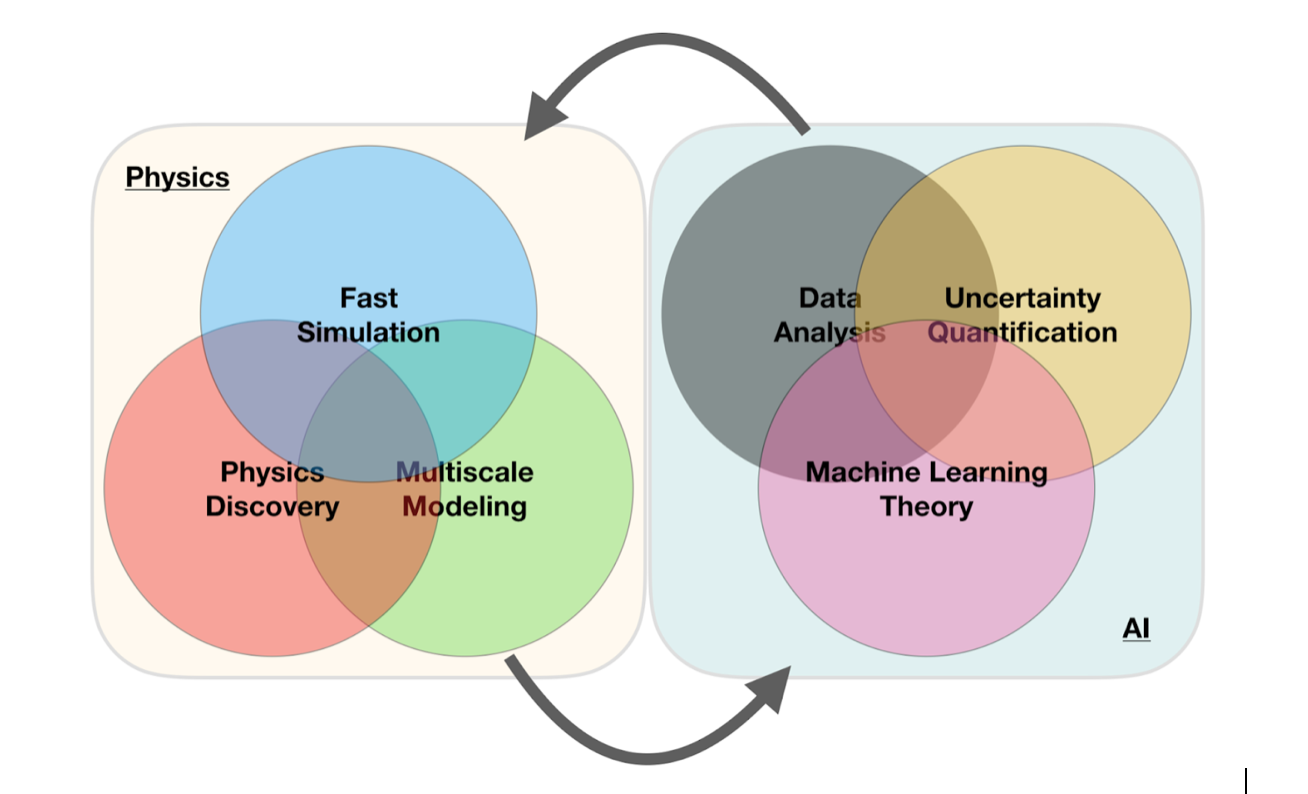
\includegraphics[width=1.0\linewidth]{figures/mlimage.png}}

\vspace{6mm}

% !split
\subsection{ML in Nuclear  Physics (or any field in physics)}

\vspace{6mm}

% inline figure
\centerline{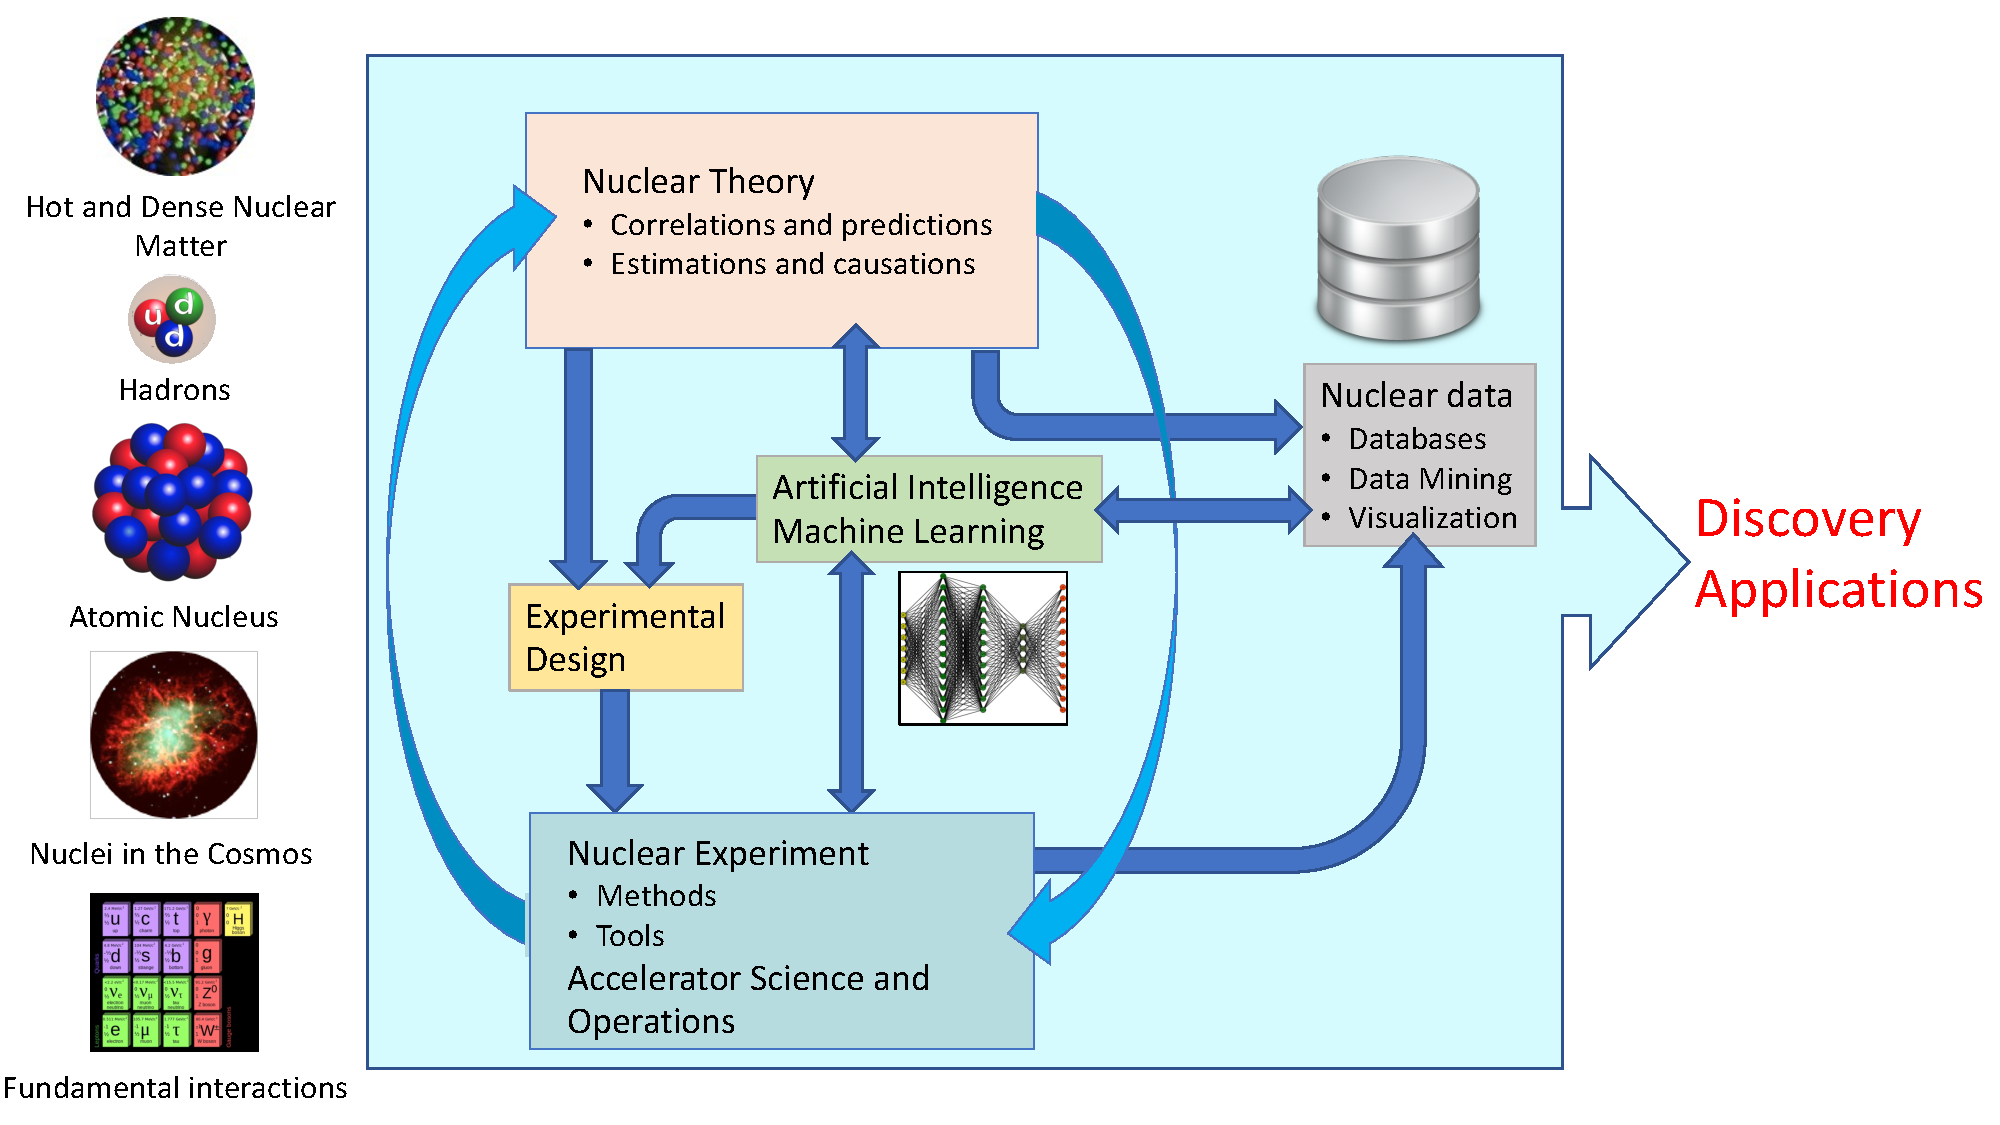
\includegraphics[width=1.0\linewidth]{figures/ML-NP.pdf}}

\vspace{6mm}

% !split
\subsection{Machine learning in physics  (my bias): Why?}

\begin{enumerate}
\item ML tools can help us to speed up the scientific process cycle and hence facilitate discoveries

\item Enabling fast emulation for big simulations

\item Revealing the information content of measured observables w.r.t. theory

\item Identifying crucial experimental data for better constraining theory

\item Providing meaningful input to applications and planned measurements

\item ML tools can help us to reveal the structure of our models

\item Parameter estimation with heterogeneous/multi-scale datasets

\item Model reduction

\item ML tools can help us to provide predictive capability

\item Theoretical results often involve ultraviolet  and infrared extrapolations due to Hilbert-space truncations 

\item Uncertainty quantification essential

\item Theoretical models are often applied to entirely new nuclear systems and conditions that are not accessible to experiment
\end{enumerate}

\noindent
% !split
\subsection{Examples of applications of ML in physics}

The large amount of degrees of freedom pertain to both theory and
experiment in physics. With increasingly complicated
experiments that produce large amounts data, automated classification
of events becomes increasingly important. 

\begin{block}{}
\begin{itemize}
\item Reconstruction of particle trajectories or classification of events are typical examples where ML methods are being used. However, since these data can often be extremely noisy, the precision necessary for discovery in physics requires algorithmic improvements. Research along such directions, interfacing nuclear physics with AI/ML is expected to play a significant role in physics discoveries related to new facilities.  The treatment of corrupted data in imaging and image processing is also a relevant topic. 

\item Design of detectors represents an important area of applications for ML/AI methods in subatomic physics.
\end{itemize}

\noindent
\end{block}

% !split
\subsection{Scientific Machine Learning}

An important and emerging field is what has been dubbed as scientific ML, see the article by Deiana et al "Applications and Techniques for Fast Machine Learning in Science, Big Data \textbf{5}, 787421 (2022):https://doi.org/10.3389/fdata.2022.787421"

\begin{block}{}
The authors discuss applications and techniques for fast machine
learning (ML) in science -- the concept of integrating power ML
methods into the real-time experimental data processing loop to
accelerate scientific discovery. The report covers three main areas

\begin{enumerate}
\item applications for fast ML across a number of scientific domains;

\item techniques for training and implementing performant and resource-efficient ML algorithms;

\item and computing architectures, platforms, and technologies for deploying these algorithms.
\end{enumerate}

\noindent
\end{block}

% !split
\subsection{ML for detectors}

\vspace{6mm}

% inline figure
\centerline{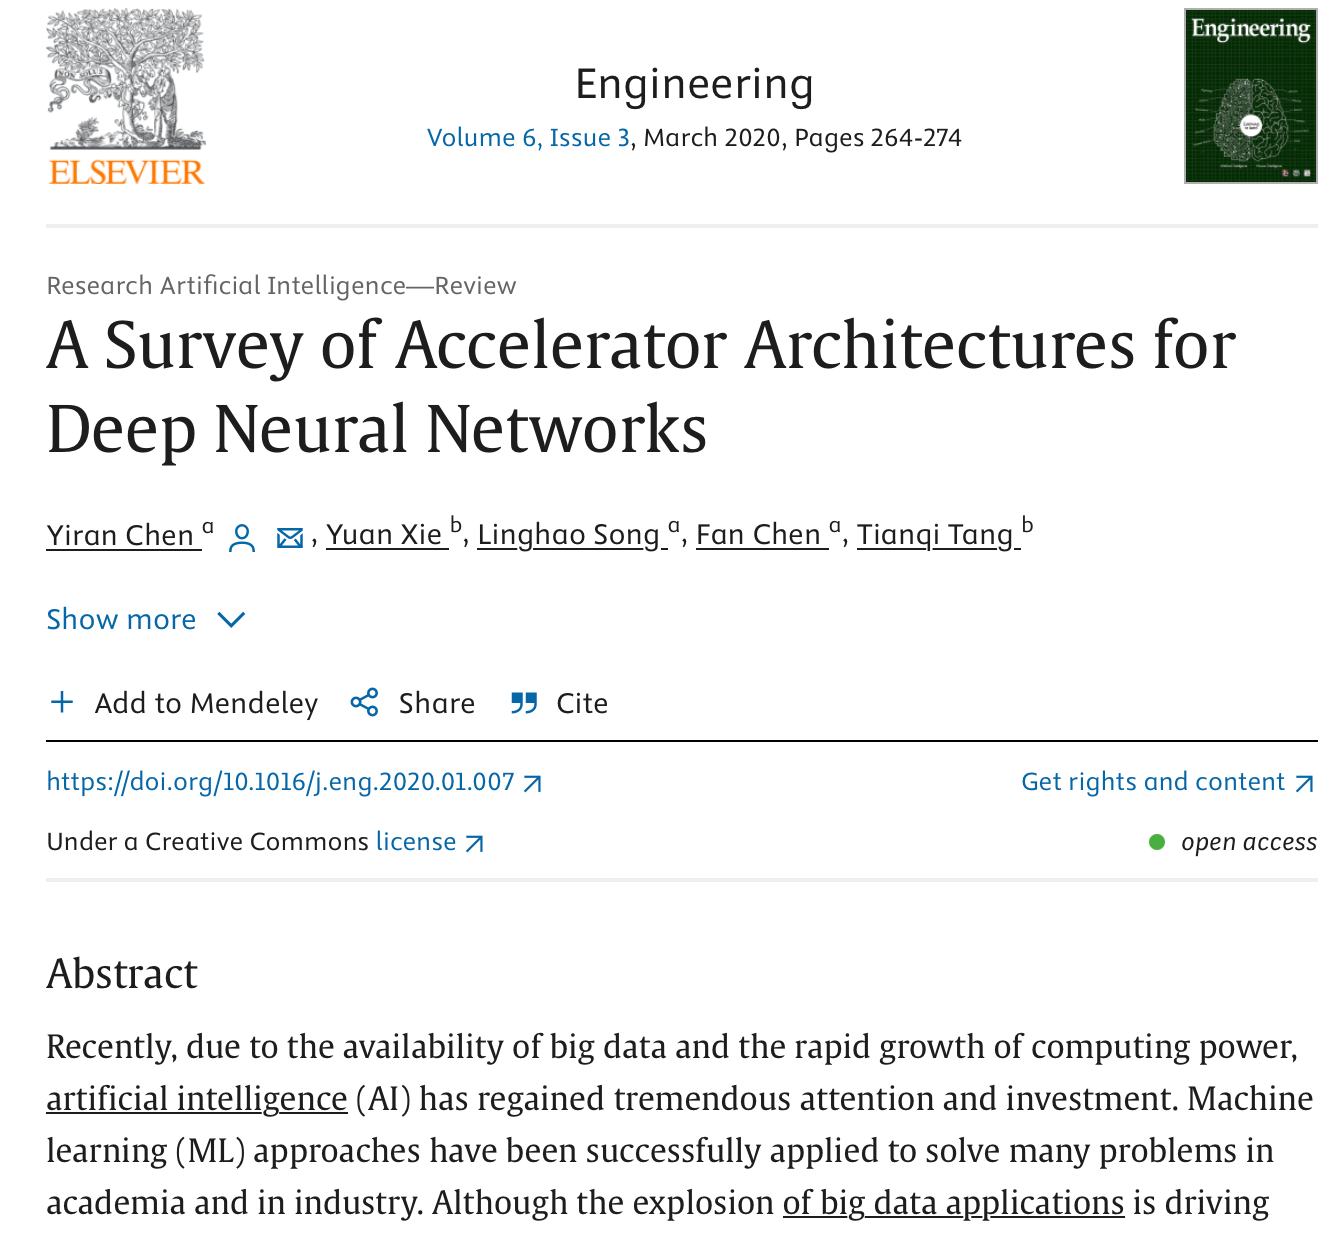
\includegraphics[width=1.0\linewidth]{figures/detectors.png}}

\vspace{6mm}

% !split
\subsection{Physics driven Machine Learning}

Another hot topic is what has loosely been dubbed \textbf{Physics-driven deep learning}. See the recent work on \href{{https://www.nature.com/articles/s42256-021-00302-5}}{Learning nonlinear operators via DeepONet based on the universal approximation theorem of operators, Nature Machine Learning, vol 3, 218 (2021)}.

\begin{block}{From their abstract }
A less known but powerful result is that an NN with a single hidden layer can accurately approximate any nonlinear continuous operator. This universal approximation theorem of operators is suggestive of the structure and potential of deep neural networks (DNNs) in learning continuous operators or complex systems from streams of scattered data. ...  We demonstrate that DeepONet can learn various explicit operators, such as integrals and fractional Laplacians, as well as implicit operators that represent deterministic and stochastic differential equations. 
\end{block}

% !split
\subsection{And more}

\begin{block}{}
\begin{itemize}
\item An important application of AI/ML methods is to improve the estimation of bias or uncertainty due to the introduction of or lack of physical constraints in various theoretical models.

\item In theory, we expect to use AI/ML algorithms and methods to improve our knowledge about  correlations of physical model parameters in data for quantum many-body systems. Deep learning methods show great promise in circumventing the exploding dimensionalities encountered in quantum mechanical many-body studies. 

\item Merging a frequentist approach (the standard path in ML theory) with a Bayesian approach, has the potential to infer better probabilitity distributions and error estimates. 

\item Machine Learning and Quantum Computing is a very interesting avenue to explore. See for example a recent talk by \href{{https://www.youtube.com/watch?v=7WPKv1Q57os&list=PLUPPQ1TVXK7uHwCTccWMBud-zLyvAf8A2&index=5&ab_channel=ECTstar}}{Sofia Vallecorsa}.
\end{itemize}

\noindent
\end{block}

% !split
\subsection{Argon-46 by Solli et al., NIMA 1010, 165461 (2021)}

\begin{block}{}
Representations of two events from the
Argon-46 experiment. Each row is one event in two projections,
where the color intensity of each point indicates higher charge values
recorded by the detector. The bottom row illustrates a carbon event with
a large fraction of noise, while the top row shows a proton event
almost free of noise. 
\end{block}

\vspace{6mm}

% inline figure
\centerline{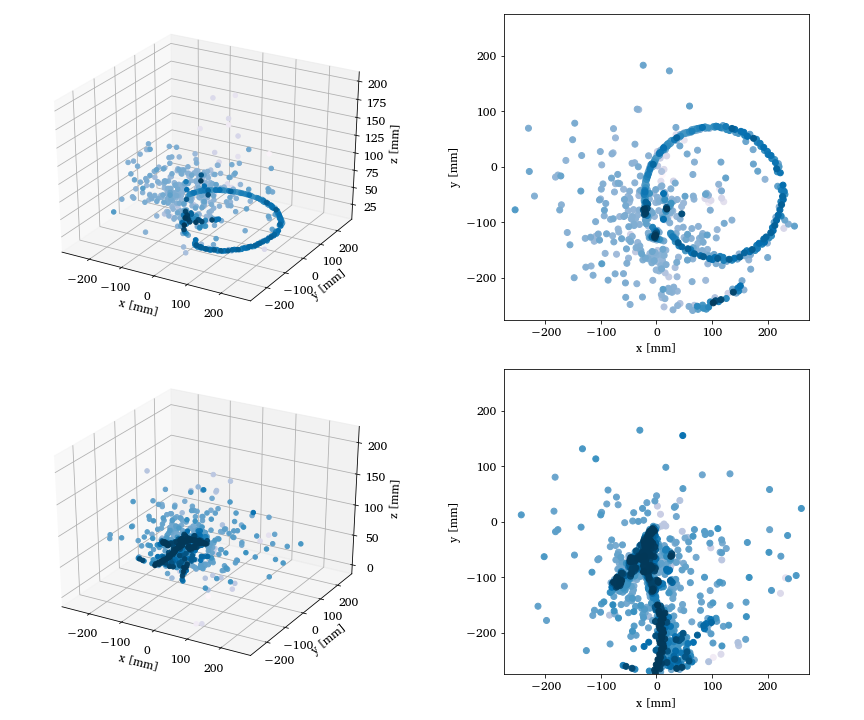
\includegraphics[width=0.6\linewidth]{figures/examples_raw.png}}

\vspace{6mm}

% !split
\subsection{Many-body physics, Quantum Monte Carlo and deep learning}
\begin{block}{}
Given a hamiltonian $H$ and a trial wave function $\Psi_T$, the variational principle states that the expectation value of $\langle H \rangle$, defined through 
\[
   \langle E \rangle =
   \frac{\int d\bm{R}\Psi^{\ast}_T(\bm{R})H(\bm{R})\Psi_T(\bm{R})}
        {\int d\bm{R}\Psi^{\ast}_T(\bm{R})\Psi_T(\bm{R})},
\]
is an upper bound to the ground state energy $E_0$ of the hamiltonian $H$, that is 
\[
    E_0 \le \langle E \rangle.
\]
In general, the integrals involved in the calculation of various  expectation values  are multi-dimensional ones. Traditional integration methods such as the Gauss-Legendre will not be adequate for say the  computation of the energy of a many-body system.  \textbf{Basic philosophy: Let a neural network find the optimal wave function}
\end{block}

% !split
\subsection{Quantum Monte Carlo Motivation}
\begin{block}{Basic steps }
Choose a trial wave function
$\psi_T(\bm{R})$.
\[
   P(\bm{R},\bm{\alpha})= \frac{\left|\psi_T(\bm{R},\bm{\alpha})\right|^2}{\int \left|\psi_T(\bm{R},\bm{\alpha})\right|^2d\bm{R}}.
\]
This is our model, or likelihood/probability distribution function  (PDF). It depends on some variational parameters $\bm{\alpha}$.
The approximation to the expectation value of the Hamiltonian is now 
\[
   \langle E[\bm{\alpha}] \rangle = 
   \frac{\int d\bm{R}\Psi^{\ast}_T(\bm{R},\bm{\alpha})H(\bm{R})\Psi_T(\bm{R},\bm{\alpha})}
        {\int d\bm{R}\Psi^{\ast}_T(\bm{R},\bm{\alpha})\Psi_T(\bm{R},\bm{\alpha})}.
\]
\end{block}

% !split
\subsection{Quantum Monte Carlo Motivation}
\begin{block}{Define a new quantity }
\[
   E_L(\bm{R},\bm{\alpha})=\frac{1}{\psi_T(\bm{R},\bm{\alpha})}H\psi_T(\bm{R},\bm{\alpha}),
\]
called the local energy, which, together with our trial PDF yields
\[
  \langle E[\bm{\alpha}] \rangle=\int P(\bm{R})E_L(\bm{R},\bm{\alpha}) d\bm{R}\approx \frac{1}{N}\sum_{i=1}^NE_L(\bm{R_i},\bm{\alpha})
\]
with $N$ being the number of Monte Carlo samples.
\end{block}

% !split
\subsection{Energy derivatives}
\begin{block}{}
The local energy as function of the variational parameters defines now our \textbf{objective/cost} function.

To find the derivatives of the local energy expectation value as function of the variational parameters, we can use the chain rule and the hermiticity of the Hamiltonian.  

Let us define (with the notation $\langle E[\bm{\alpha}]\rangle =\langle  E_L\rangle$)
\[
\bar{E}_{\alpha_i}=\frac{d\langle  E_L\rangle}{d\alpha_i},
\]
as the derivative of the energy with respect to the variational parameter $\alpha_i$
We define also the derivative of the trial function (skipping the subindex $T$) as 
\[
\bar{\Psi}_{i}=\frac{d\Psi}{d\alpha_i}.
\]
\end{block}

% !split
\subsection{Derivatives of the local energy}
\begin{block}{}
The elements of the gradient of the local energy are 
\[
\bar{E}_{i}= 2\left( \langle \frac{\bar{\Psi}_{i}}{\Psi}E_L\rangle -\langle \frac{\bar{\Psi}_{i}}{\Psi}\rangle\langle E_L \rangle\right).
\]
From a computational point of view it means that you need to compute the expectation values of 
\[
\langle \frac{\bar{\Psi}_{i}}{\Psi}E_L\rangle,
\]
and
\[
\langle \frac{\bar{\Psi}_{i}}{\Psi}\rangle\langle E_L\rangle
\]
These integrals are evaluted using MC intergration (with all its possible error sources). Use methods like stochastic gradient or other minimization methods to find the optimal parameters.
\end{block}

% !split
\subsection{Why Feed Forward Neural Networks?}

According to the \emph{Universal approximation theorem}, a feed-forward
neural network with just a single hidden layer containing a finite
number of neurons can approximate a continuous multidimensional
function to arbitrary accuracy, assuming the activation function for
the hidden layer is a \textbf{non-constant, bounded and
monotonically-increasing continuous function}.

% !split
\subsection{Illustration of a single perceptron model and a multi-perceptron model}

\begin{figure}[!ht]  % 
  \centerline{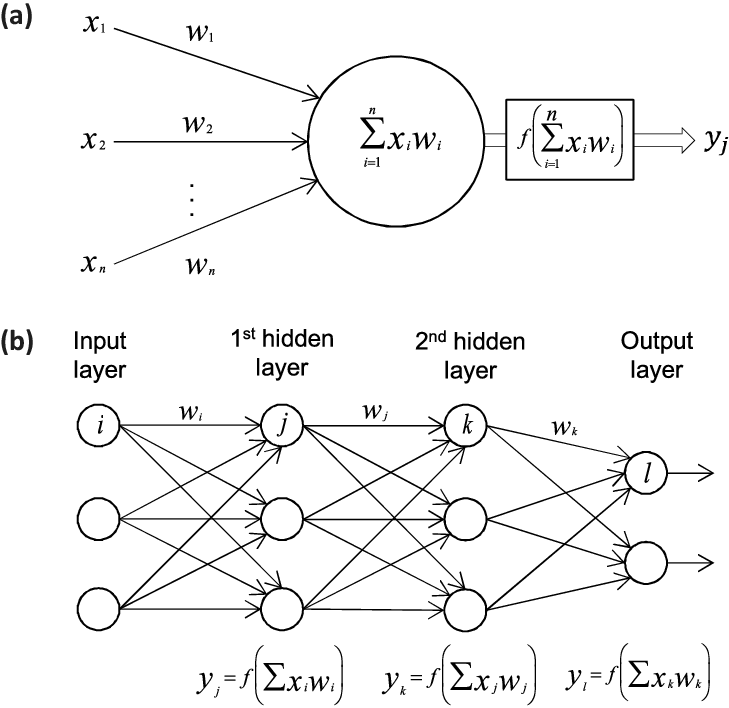
\includegraphics[width=0.8\linewidth]{figures/nns.png}}
  \caption{
  In a) we show a single perceptron model while in b) we dispay a network with two  hidden layers, an input layer and an output layer.
  }
\end{figure}
%\clearpage % flush figures 

% !split
\subsection{Monte Carlo methods and Neural Networks}

\href{{https://www.sciencedirect.com/science/article/pii/S0370269320305463?via%3Dihub}}{Machine Learning and the Deuteron by Kebble and Rios} and
\href{{https://journals.aps.org/prl/abstract/10.1103/PhysRevLett.127.022502}}{Variational Monte Carlo calculations of $A\le 4$ nuclei with an artificial neural-network correlator ansatz by Adams et al.}

\textbf{Adams et al}:

\begin{align}
H_{LO} &=-\sum_i \frac{{\vec{\nabla}_i^2}}{2m_N}
+\sum_{i<j} {\left(C_1  + C_2\, \vec{\sigma_i}\cdot\vec{\sigma_j}\right)
e^{-r_{ij}^2\Lambda^2 / 4 }}
\nonumber\\
&+D_0 \sum_{i<j<k} \sum_{\text{cyc}}
{e^{-\left(r_{ik}^2+r_{ij}^2\right)\Lambda^2/4}}\,,
\end{align}

where $m_N$ is the mass of the nucleon, $\vec{\sigma_i}$ is the Pauli
matrix acting on nucleon $i$, and $\sum_{\text{cyc}}$ stands for the
cyclic permutation of $i$, $j$, and $k$. The low-energy constants
$C_1$ and $C_2$ are fit to the deuteron binding energy and to the
neutron-neutron scattering length

% !split
\subsection{Deep learning neural networks, \href{{https://journals.aps.org/prl/abstract/10.1103/PhysRevLett.127.022502}}{Variational Monte Carlo calculations of $A\le 4$ nuclei with an artificial neural-network correlator ansatz by Adams et al.}}

An appealing feature of the neural network ansatz is that it is more general than the more conventional product of two-
and three-body spin-independent Jastrow functions
\begin{align}
|\Psi_V^J \rangle = \prod_{i<j<k} \Big( 1-\sum_{\text{cyc}} u(r_{ij}) u(r_{jk})\Big) \prod_{i<j} f(r_{ij}) | \Phi\rangle\,,
\end{align}
which is commonly used for nuclear Hamiltonians that do not contain tensor and spin-orbit terms.
The above function is replaced by a four-layer Neural Network. 

% !split
\subsection{\href{{https://journals.aps.org/prresearch/pdf/10.1103/PhysRevResearch.5.033062}}{Dilute neutron star matter from neural-network quantum states by Fore et al, Physical Review Research 5, 033062 (2023)} at density $\rho=0.04$ fm$^{-3}$}

\begin{block}{}

\vspace{6mm}

% inline figure
\centerline{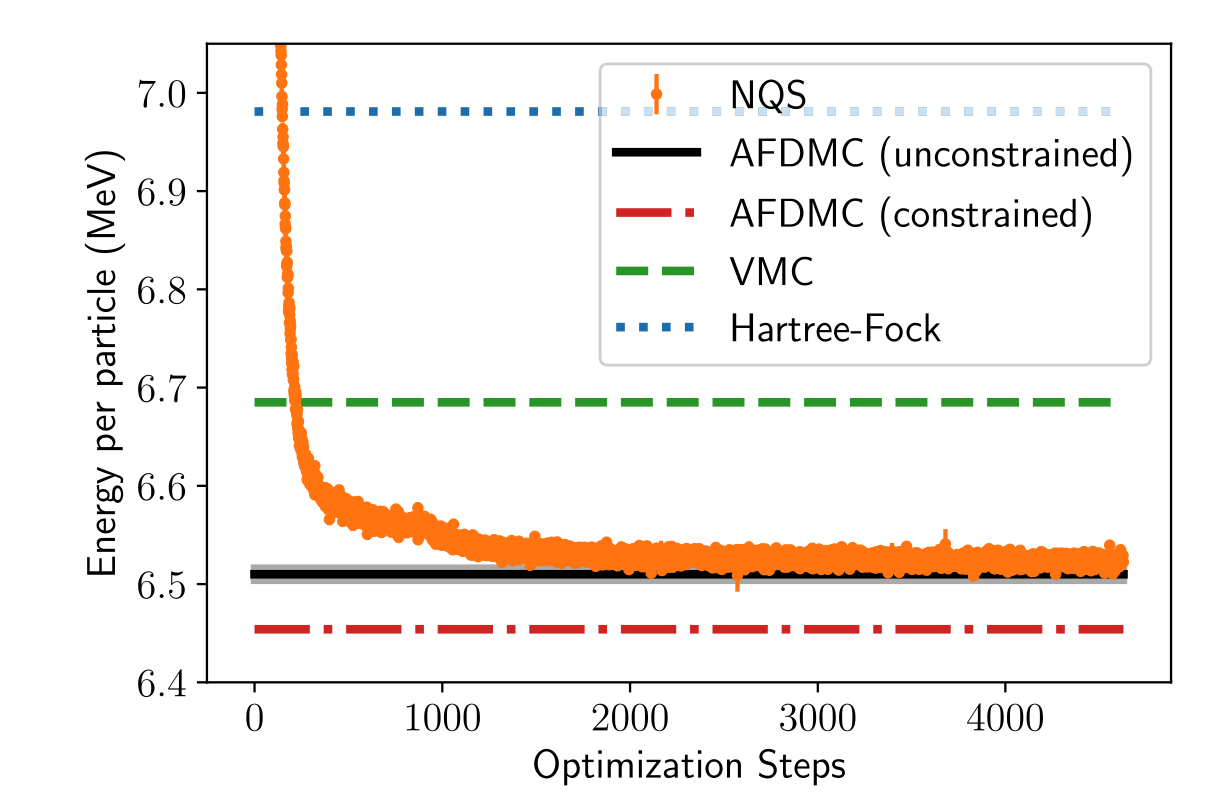
\includegraphics[width=0.9\linewidth]{figures/nmatter.png}}

\vspace{6mm}

\end{block}

% !split

\subsection{Pairing and Spin-singlet and triplet two-body distribution functions at $\rho=0.01$ fm$^{-3}$}
\begin{block}{}

\vspace{6mm}

% inline figure
\centerline{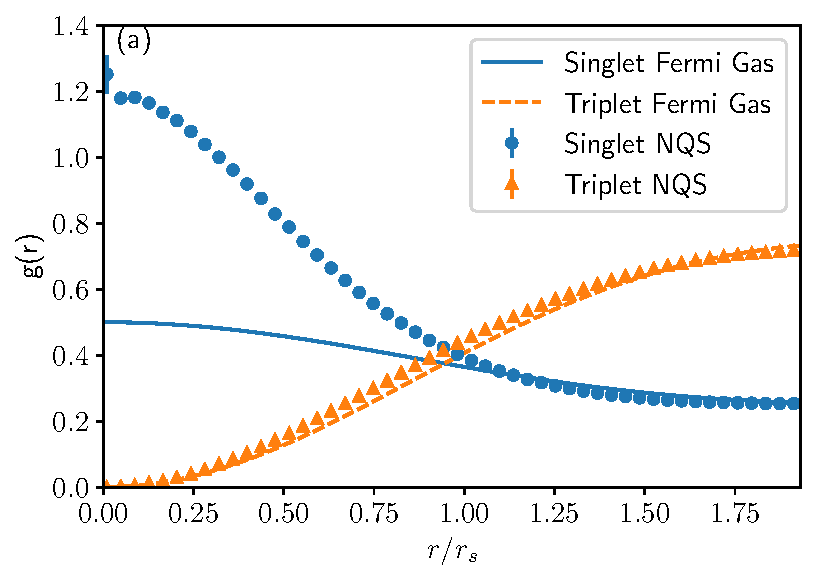
\includegraphics[width=0.9\linewidth]{figures/01_tbd.pdf}}

\vspace{6mm}

\end{block}

% !split
\subsection{Pairing and Spin-singlet and triplet two-body distribution functions at $\rho=0.04$ fm$^{-3}$}

\begin{block}{}

\vspace{6mm}

% inline figure
\centerline{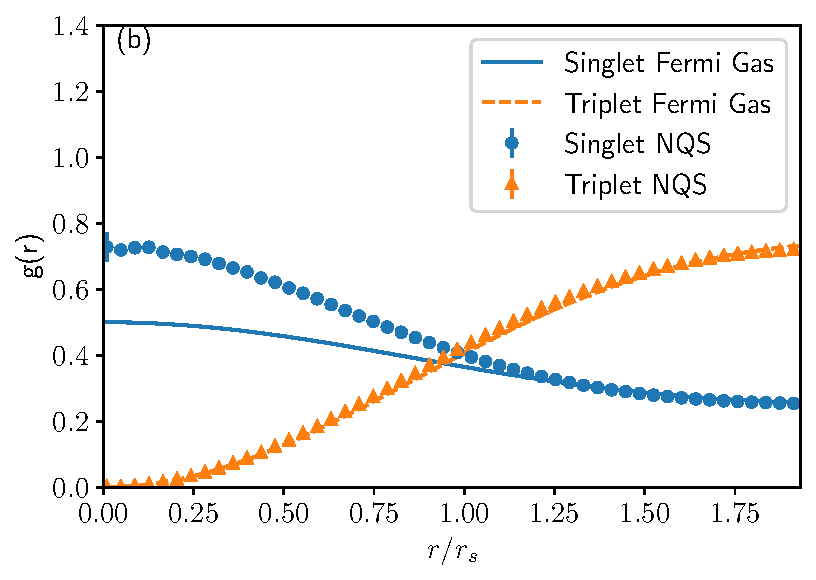
\includegraphics[width=0.9\linewidth]{figures/04_tbd.pdf}}

\vspace{6mm}

\end{block}

% !split
\subsection{Pairing and Spin-singlet and triplet two-body distribution functions at $\rho=0.08$ fm$^{-3}$}
\begin{block}{}

\vspace{6mm}

% inline figure
\centerline{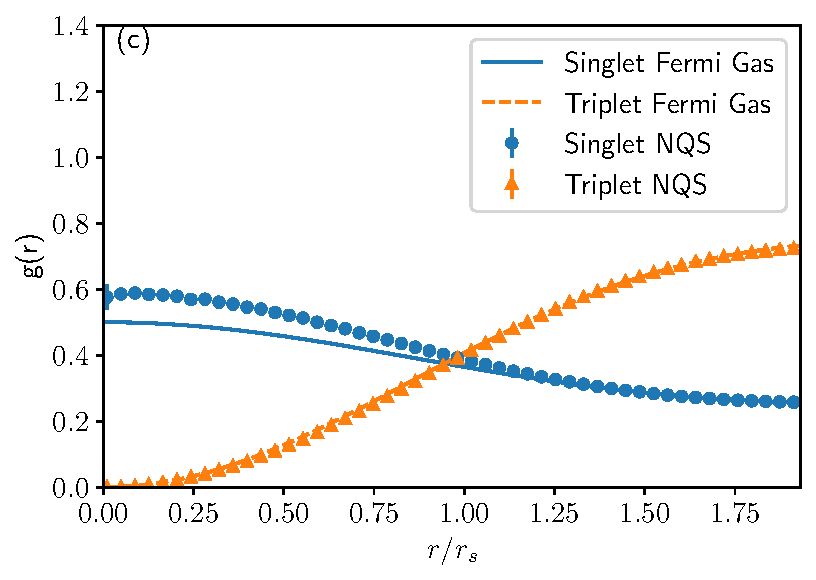
\includegraphics[width=0.9\linewidth]{figures/08_tbd.pdf}}

\vspace{6mm}

\end{block}

% !split
\subsection{The electron gas in three dimensions with $N=14$ electrons (Wigner-Seitz radius $r_s=2$ a.u.), \href{{https://doi.org/10.48550/arXiv.2305.07240}}{Gabriel Pescia, Jane Kim et al.~arXiv.2305.07240,}}

\begin{block}{}

\vspace{6mm}

% inline figure
\centerline{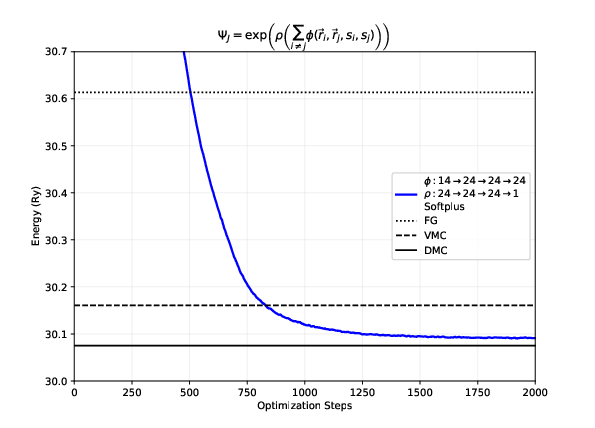
\includegraphics[width=0.9\linewidth]{figures/elgasnew.png}}

\vspace{6mm}

\end{block}

% !split
\subsection{\href{{https://doi.org/10.3389/fphy.2023.1061580}}{Efficient solutions of fermionic systems using artificial neural networks, Nordhagen et al, Frontiers in Physics 11, 2023}}

The Hamiltonian of the quantum dot is given by
\[ \hat{H} = \hat{H}_0 + \hat{V}, 
\]
where $\hat{H}_0$ is the many-body HO Hamiltonian, and $\hat{V}$ is the
inter-electron Coulomb interactions. In dimensionless units,
\[ \hat{V}= \sum_{i < j}^N \frac{1}{r_{ij}},
\]
with $r_{ij}=\sqrt{\mathbf{r}_i^2 - \mathbf{r}_j^2}$.

Separable Hamiltonian with the relative motion part ($r_{ij}=r$)
\[ 
\hat{H}_r=-\nabla^2_r + \frac{1}{4}\omega^2r^2+ \frac{1}{r},
\]
Analytical solutions in two and three dimensions (\href{{https://journals.aps.org/pra/abstract/10.1103/PhysRevA.48.3561}}{M. Taut 1993 and 1994}). 

% !split
\subsection{Quantum dots and Boltzmann machines, onebody densities $N=6$, $\hbar\omega=0.1$ a.u.}

\begin{block}{}

\vspace{6mm}

% inline figure
\centerline{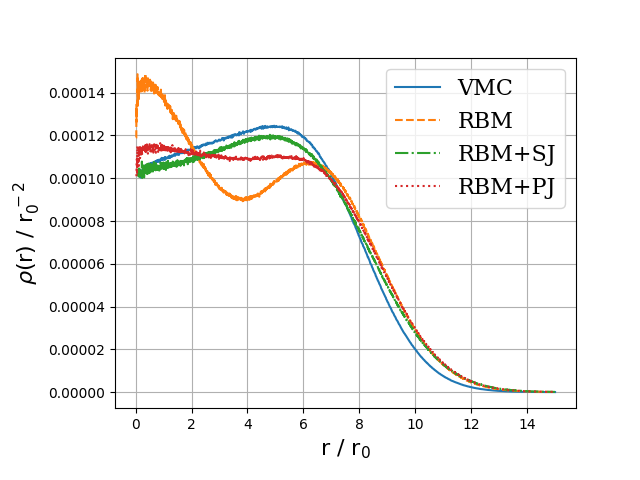
\includegraphics[width=0.9\linewidth]{figures/OB6hw01.png}}

\vspace{6mm}

\end{block}

% !split
\subsection{Onebody densities $N=30$, $\hbar\omega=1.0$ a.u.}
\begin{block}{}

\vspace{6mm}

% inline figure
\centerline{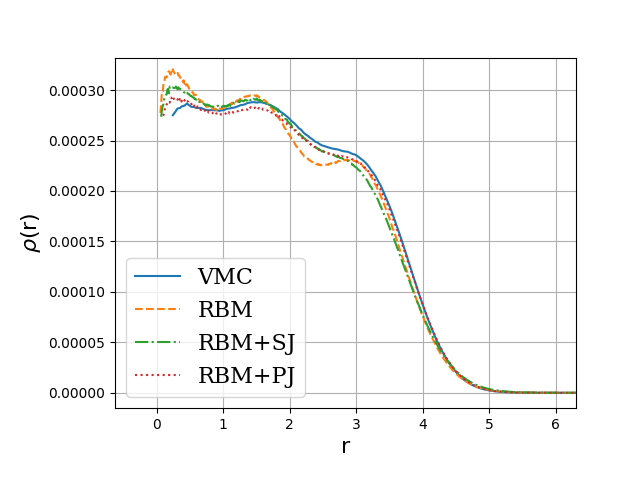
\includegraphics[width=0.9\linewidth]{figures/OB30hw1.png}}

\vspace{6mm}

\end{block}

% !split
\subsection{Onebody densities $N=30$, $\hbar\omega=0.1$ a.u.}
\begin{block}{}

\vspace{6mm}

% inline figure
\centerline{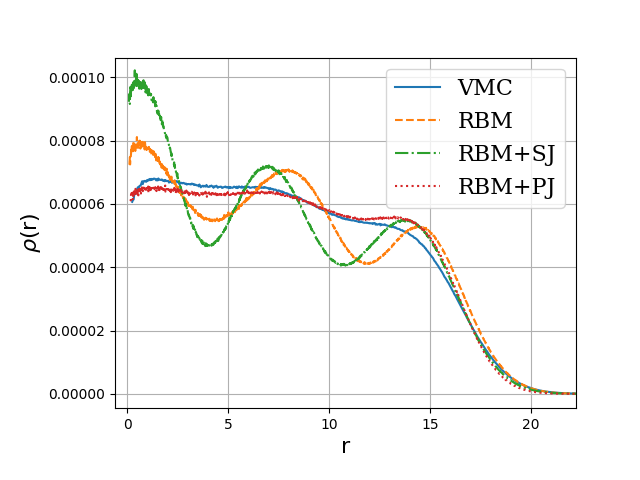
\includegraphics[width=0.9\linewidth]{figures/OB30hw01.png}}

\vspace{6mm}

\end{block}

% !split
\subsection{Extrapolations and model interpretability}

When you hear phrases like \textbf{predictions and estimations} and
\textbf{correlations and causations}, what do you think of?  May be you think
of the difference between classifying new data points and generating
new data points.
Or perhaps you consider that correlations represent some kind of symmetric statements like
if $A$ is correlated with $B$, then $B$ is correlated with
$A$. Causation on the other hand is directional, that is if $A$ causes $B$, $B$ does not
necessarily cause $A$.

% !split
\subsection{Physics based statistical learning and data analysis}

The above concepts are in some sense the difference between \textbf{old-fashioned} machine
learning and statistics and Bayesian learning. In machine learning and prediction based
tasks, we are often interested in developing algorithms that are
capable of learning patterns from given data in an automated fashion,
and then using these learned patterns to make predictions or
assessments of newly given data. In many cases, our primary concern
is the quality of the predictions or assessments, and we are less
concerned about the underlying patterns that were learned in order
to make these predictions.

Physics based statistical learning points however to approaches that give us both predictions and correlations as well as being able to produce error estimates and understand causations.  This leads us to the very interesting field of Bayesian statistics.

% !split
\subsection{Bayes' Theorem}

Bayes' theorem
\[
p(X\vert Y)= \frac{p(X,Y)}{\sum_{i=0}^{n-1}p(Y\vert X=x_i)p(x_i)}=\frac{p(Y\vert X)p(X)}{\sum_{i=0}^{n-1}p(Y\vert X=x_i)p(x_i)}.
\]

The quantity $p(Y\vert X)$ on the right-hand side of the theorem is
evaluated for the observed data $Y$ and can be viewed as a function of
the parameter space represented by $X$. This function is not
necessarily normalized and is normally called the likelihood function.

The function $p(X)$ on the right hand side is called the prior while the function on the left hand side is the called the posterior probability. The denominator on the right hand side serves as a normalization factor for the posterior distribution.

% !split
\subsection{\href{{https://journals.aps.org/prc/abstract/10.1103/PhysRevC.101.044307}}{Quantified limits of the nuclear landscape}}

Predictions made with eleven global mass model and Bayesian model averaging

\vspace{6mm}

% inline figure
\centerline{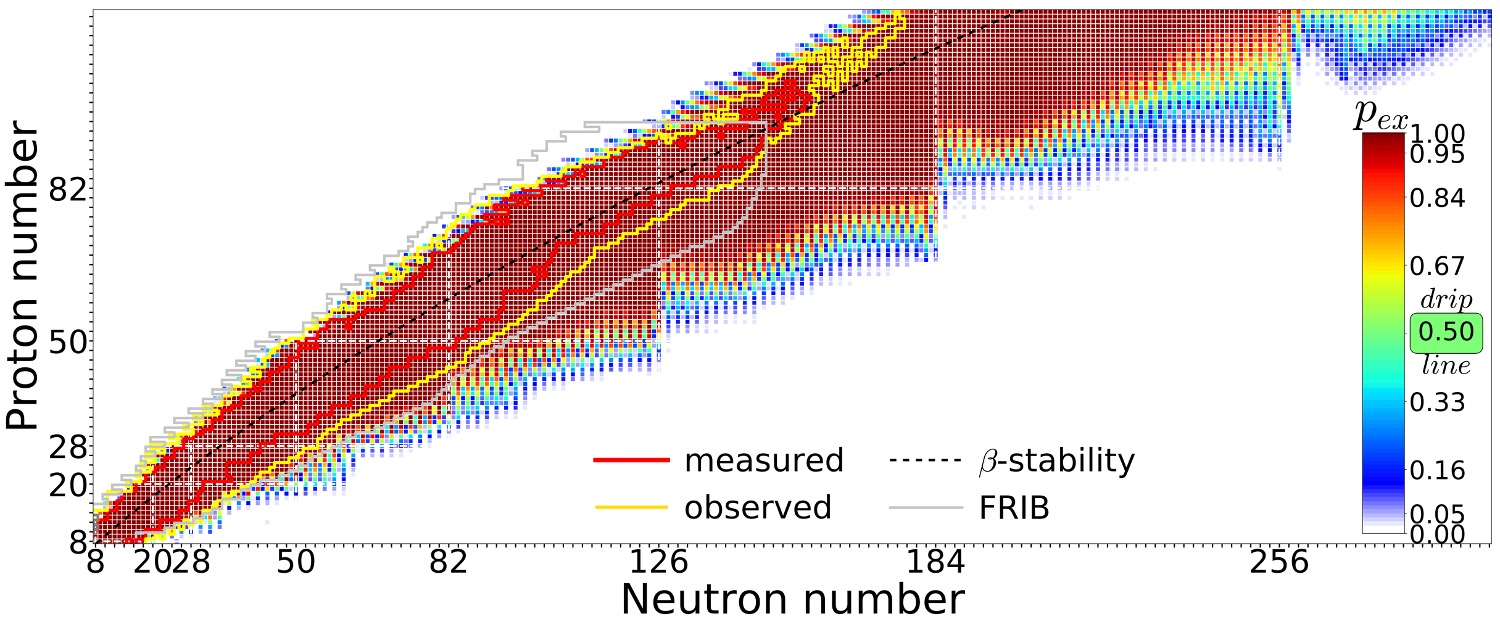
\includegraphics[width=1.0\linewidth]{figures/landscape.jpg}}

\vspace{6mm}

% !split
\subsection{Observations (or conclusions if you prefer)}
\begin{block}{}
\begin{itemize}
\item Need for AI/Machine Learning in physics, lots of ongoing activities

\item To solve many complex problems and facilitate discoveries, multidisciplinary efforts efforts are required involving scientists in  physics, statistics, computational science, applied math and other fields.

\item There is a need for  focused AI/ML learning efforts that will benefit accelerator science and experimental and theoretical programs
\end{itemize}

\noindent
\end{block}

% !split
\subsection{More observations}
\begin{block}{}
\begin{itemize}
\item How do we develop insights, competences, knowledge in statistical learning that can advance a given field?
\begin{itemize}

  \item For example: Can we use ML to find out which correlations are relevant and thereby diminish the dimensionality problem in standard many-body  theories?

  \item Can we use AI/ML in detector analysis, accelerator design, analysis of experimental data and more?

  \item Can we use AL/ML to carry out reliable extrapolations by using current experimental knowledge and current theoretical models?

\end{itemize}

\noindent
\item The community needs to invest in relevant educational efforts and training of scientists with knowledge in AI/ML. These are great challenges to the CS and DS communities

\item Quantum computing and quantum machine learning not discussed here

\item Most likely tons of things I have forgotten
\end{itemize}

\noindent
\end{block}

% !split
\subsection{Possible start to raise awareness about ML in your own field}
\begin{block}{}
\begin{itemize}
\item Make an ML challenge in your own field a la \href{{https://home.cern/news/news/computing/higgs-boson-machine-learning-challenge}}{Learning to discover: the Higgs boson machine learning challenge}. Alternatively go to kaggle.com at \href{{https://www.kaggle.com/c/higgs-boson}}{\nolinkurl{https://www.kaggle.com/c/higgs-boson}}

\item HEP@CERN and HEP in general have made significant impacts in the field of machine learning and AI. Something to learn from
\end{itemize}

\noindent
\end{block}

% !split
\subsection{Education}

\begin{enumerate}
\item Incorporate elements of statistical data analysis and Machine Learning in undergraduate programs

\item Develop courses on Machine Learning and statistical data analysis

\item Build up a series of courses in Quantum Information Technologies (QIT)

\item Modifying contents of present Physics programs or new programs on  Computational Physics and Quantum Technologies
\begin{enumerate}

 \item study direction/option in \textbf{quantum technologies}

 \item study direction/option in \textbf{Artificial Intelligence and Machine Learning}

 \item and more

\end{enumerate}

\noindent
\item Master of Science/PhD programs in Computational and Data Science
\begin{enumerate}

 \item UiO has already MSc programs in CS and DS

 \item MSU has own graduate programs plus dual degree programs in CS and DS

 \item Many other universities are developing or have similar programs
\end{enumerate}

\noindent
\end{enumerate}

\noindent
% !split
\subsection{Possible courses}

\begin{block}{Topics  in a Bachelor of Science/Master of Science }
\begin{enumerate}
\item General university course on quantum mech and quantum technologies

\item Information Systems 

\item From Classical Information theory to Quantum Information theory

\item Classical vs.~Quantum Logic

\item Classical and Quantum Laboratory 

\item Discipline-Based Quantum Mechanics 

\item Quantum Software

\item Quantum Hardware

\item more
\end{enumerate}

\noindent
\end{block}

% !split
\subsection{Important Issues to think of}

\begin{enumerate}
\item Lots of conceptual learning: superposition, entanglement, QIT applications, etc.

\item Coding is indispensable. 

\item Teamwork, project management, and communication are important and highly valued

\item Engagement with industry: guest lectures, virtual tours, co-ops, and/or internships.
\end{enumerate}

\noindent
% !split
\subsection{Observations}

\begin{enumerate}
\item Students do not really know what QIT is.

\item ML/AI seen as black boxes/magic!

\item Students perceive that a graduate degree is necessary to work in QIS. A BSc will help.
\end{enumerate}

\noindent
% !split
\subsection{Future Needs/Problems}

\begin{enumerate}
\item There are already  great needs for specialized people (Ph. D. s, postdocs), but also needs of  people with a broad overview of what is possible in ML/AI and/or QIT.

\item There are not enough potential employees in AI/ML and QIT . It is a supply gap, not a skills gap.

\item A BSc with specialization  is a good place to start

\item It is tremendously important to get everyone speaking the same language. Facility with the vernacular of quantum mechanics is a big plus.

\item There is a huge list of areas where technical expertise may be important. But employers are often more concerned with attributes like project management, working well in a team, interest in the field, and adaptability than in specific technical skills.
\end{enumerate}

\noindent

% ------------------- end of main content ---------------

% #ifdef PREAMBLE
\end{document}
% #endif

